\documentclass{article}
\usepackage[utf8]{inputenc}
\usepackage{listings}

\title{Skanner for kviteringer}
\author{Sivert M. Skarning}
\date{Mars 2019}

\usepackage{natbib}
\usepackage{graphicx}

\begin{document}

\maketitle

\section{Introduksjon}
Som et prosjekt i faget bildebehandling og mønstergjenkjenning ved Høgskolen i Østfold har jeg valgt å utvikle en digital kvitteringskanner. En kvitteringskanner er et program som ved hjelp av et kamera klarer å konvertere en kvittering fra fysisk til digital form. I figur \ref{fig:kvittering} ser vi et utdrag fra en kvittering.

\begin{figure}[h]
\centering
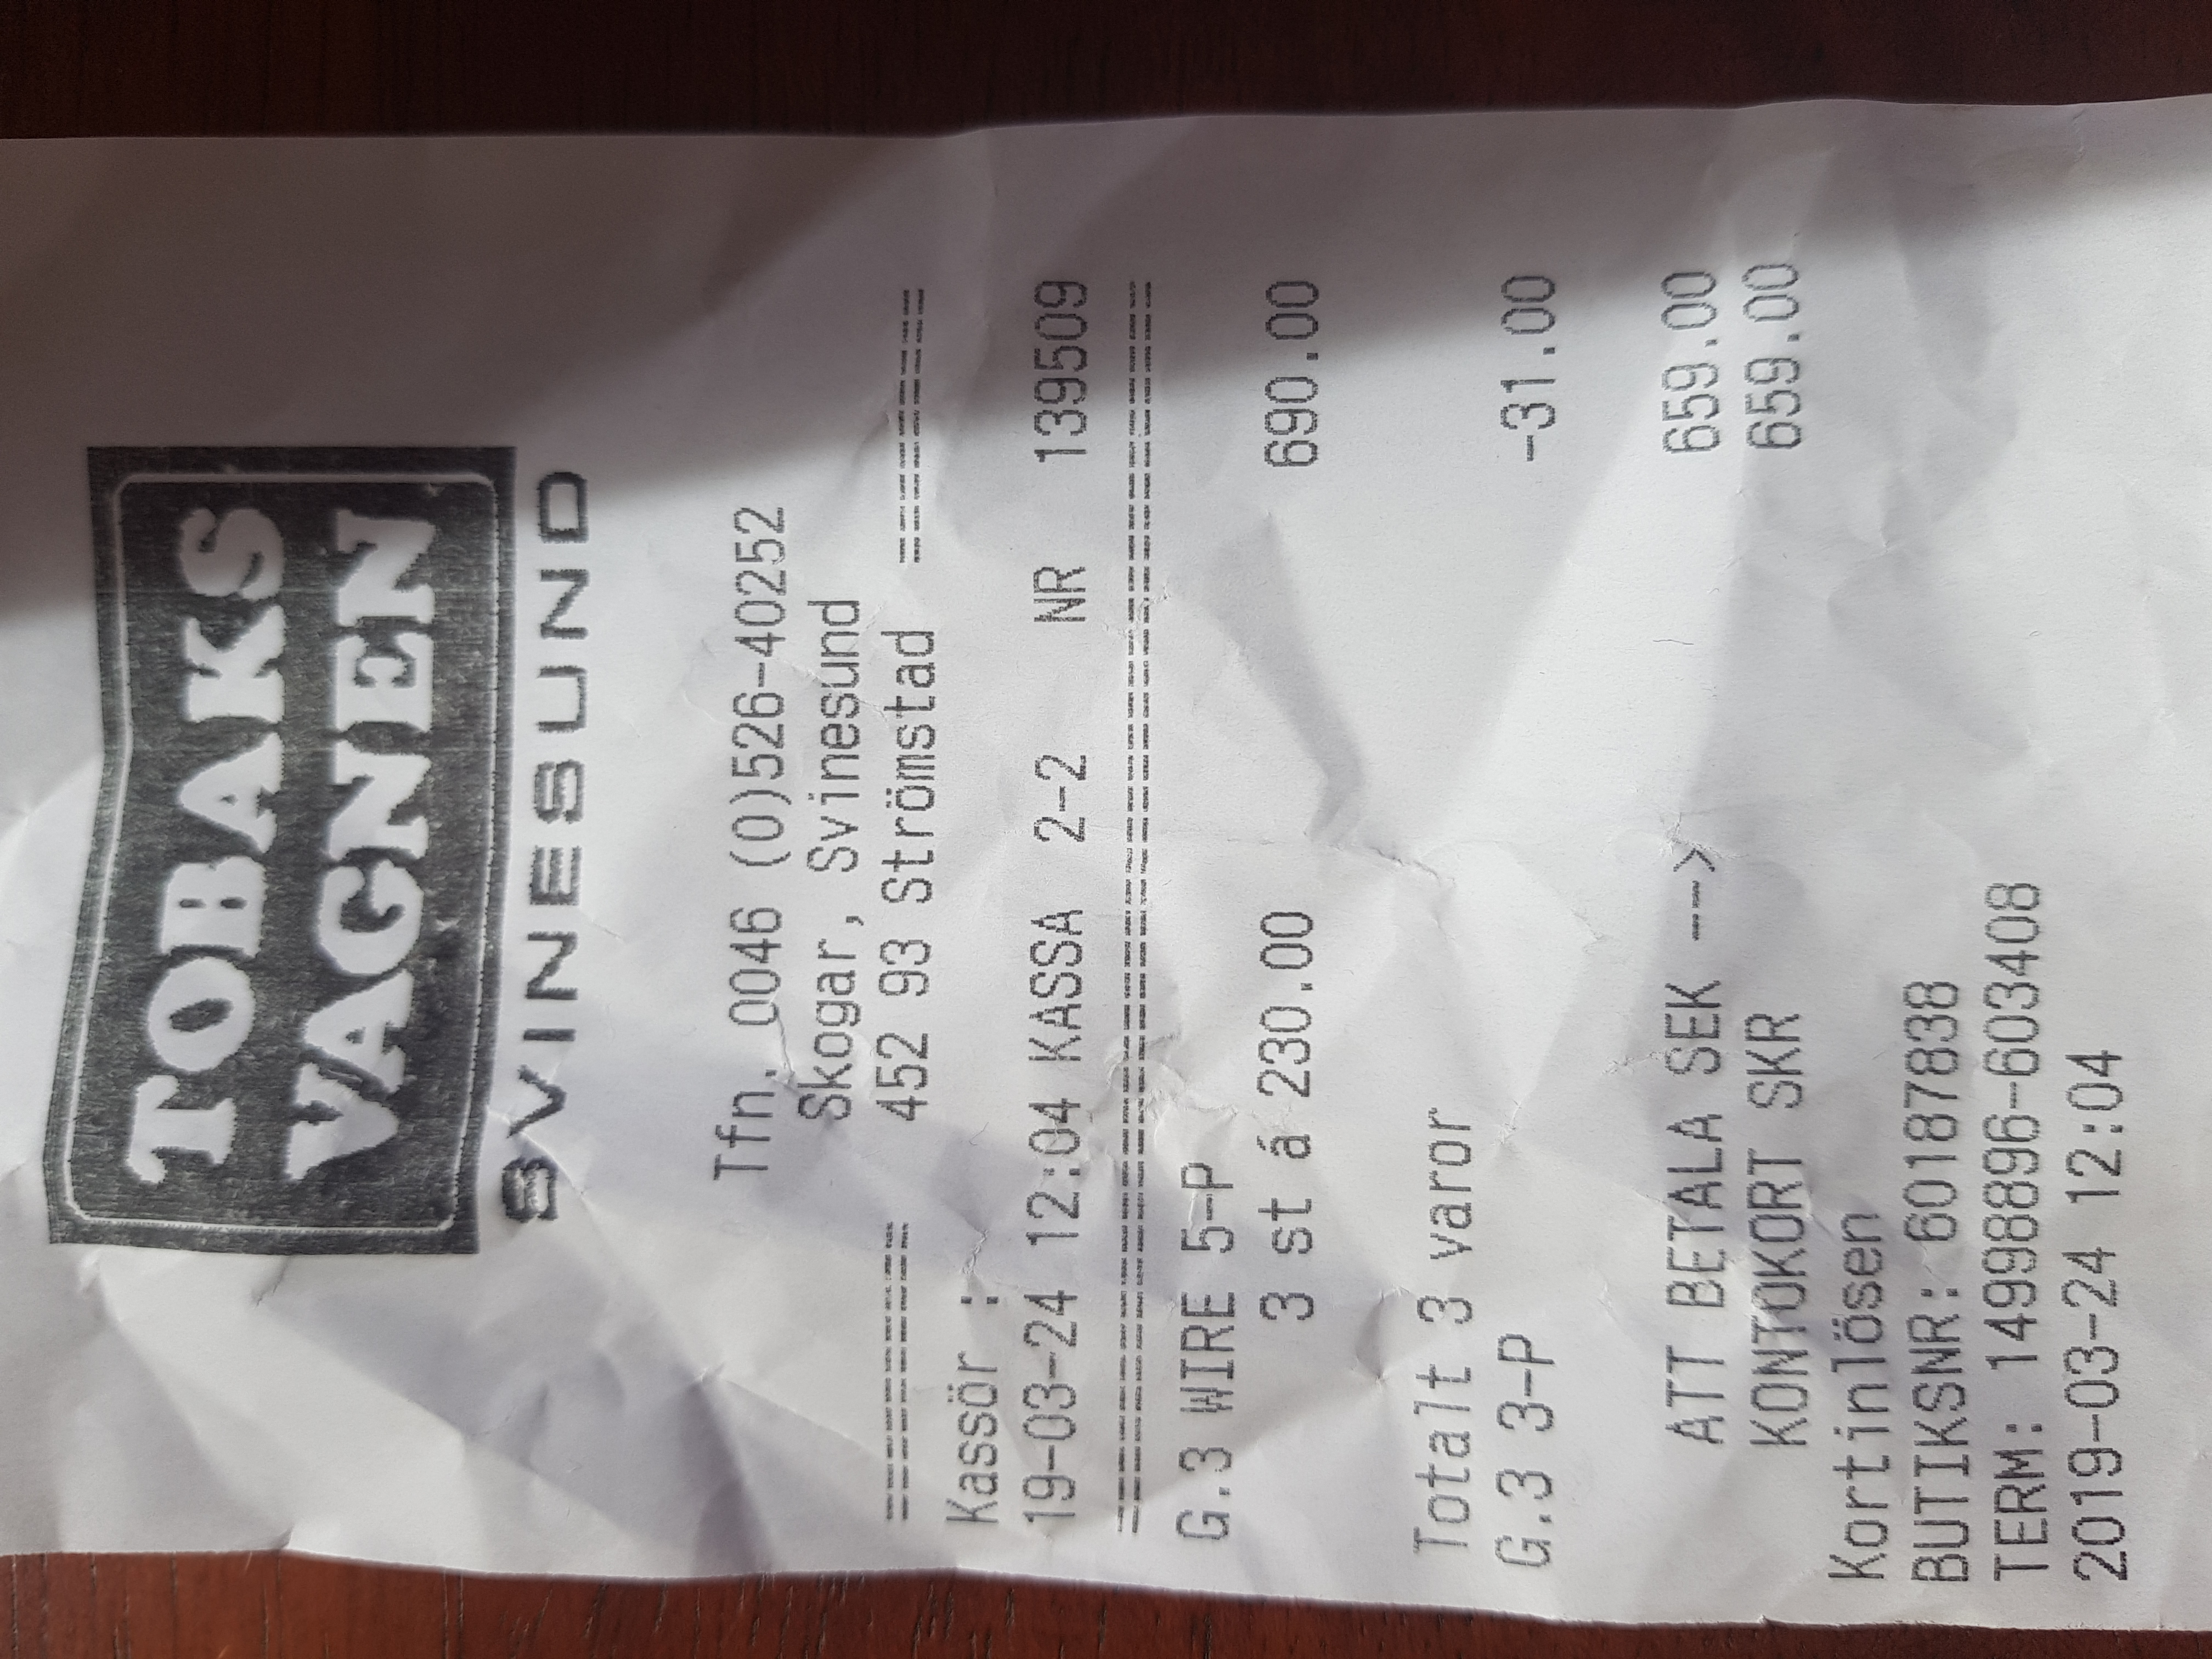
\includegraphics[scale=0.05, angle=-90]{images/kvittering.jpg}
\caption{Eksempel på en kvittering fra en svensk butikk}
\label{fig:kvittering}
\end{figure}

\section{Oppgave}
I dette prosjektet vil vi kun se på teknologien bak analysen av bilde. Det vil ikke inneholde beskrivelse av hva som skjer før og etter denne analysen, som hvordan man får inn bilde som input eller hvordan teksten blir fremvist. Oppgaven blir dermed å få inn et bilde av en kvittering finne ut hva som har blitt kjøpt, prisen, hvor produktet er blitt kjøpt, avslag og eventuelle skatter som har blitt betalt på produktet. Prosjektet kommer til å bruke kodebiblotek og eksisterende teknologier, men egen programkode skal styre retting og behandling av bilde.

\section{Teknologi}
Det finnes mange teknologier innenfor bildebehandling og tekstgjenkjenning. Jeg vil i dette prosjektet fokusere på å velge det som er enklest og implementere og open-source programvare der det er tilgjengelig.
\subsubsection{Tekstegjenkjenning}
Tesseract er et open-source programvare som utfører tekstegjenkjenning. Den kan utfører tekstgjennkjenning på mange typer filformater. Den har også API'er som gjør at det er mulig å bruke det med Python og andre programmeringspråk \footnote{https://www.learnopencv.com/deep-learning-based-text-recognition-ocr-using-tesseract-and-opencv/}. I figur \ref{fig:tesseract_output} ser dere output som blir generert etter å ha skannet bilde i figur \ref{fig:behandlet_kvittering}

\begin{figure}[h]
\centering
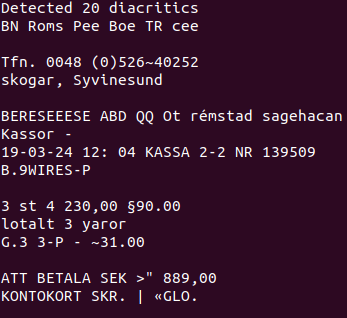
\includegraphics[scale=0.5]{images/output.png}
\caption{Output generert av Tesseract}
\label{fig:tesseract_output}
\end{figure}

\paragraph{Deskewing}
For at bilde skal kunne bli analysert på riktig måte, er vi nødt til skalere, kroppe og rotere bilde. Rotering av bilde kan bli gjort med et konsept som kalles homography. Her kan man bruke referansepunkter på et annet bilde til å rette det. Skalering og kropping er det mulig å programmere selv, eller bruke innebygde funksjoner i scikit-image. \footnote{https://www.learnopencv.com/image-alignment-feature-based-using-opencv-c-python/}
\paragraph{Oppskarpning}
Det kan være utfordrende for tekstgjenkjennings-algoritmer å kjenne igjen tekst. De fleste programmer som kjører tekstgjenkjenning kjører egne filtre for å optimaliser det for tekstgjenkjenning. For å få mer kontroll og øke sjansen for å at gjenkjenningen blir nøyaktig vil jeg bruke min egen optimerer. Den skal kunne gjøre bilde monokromt, fjerne støy, gjøre bilde skarpere og forbedre kontrasten.\footnote{https://docparser.com/blog/improve-ocr-}
\begin{figure}[h]
\centering
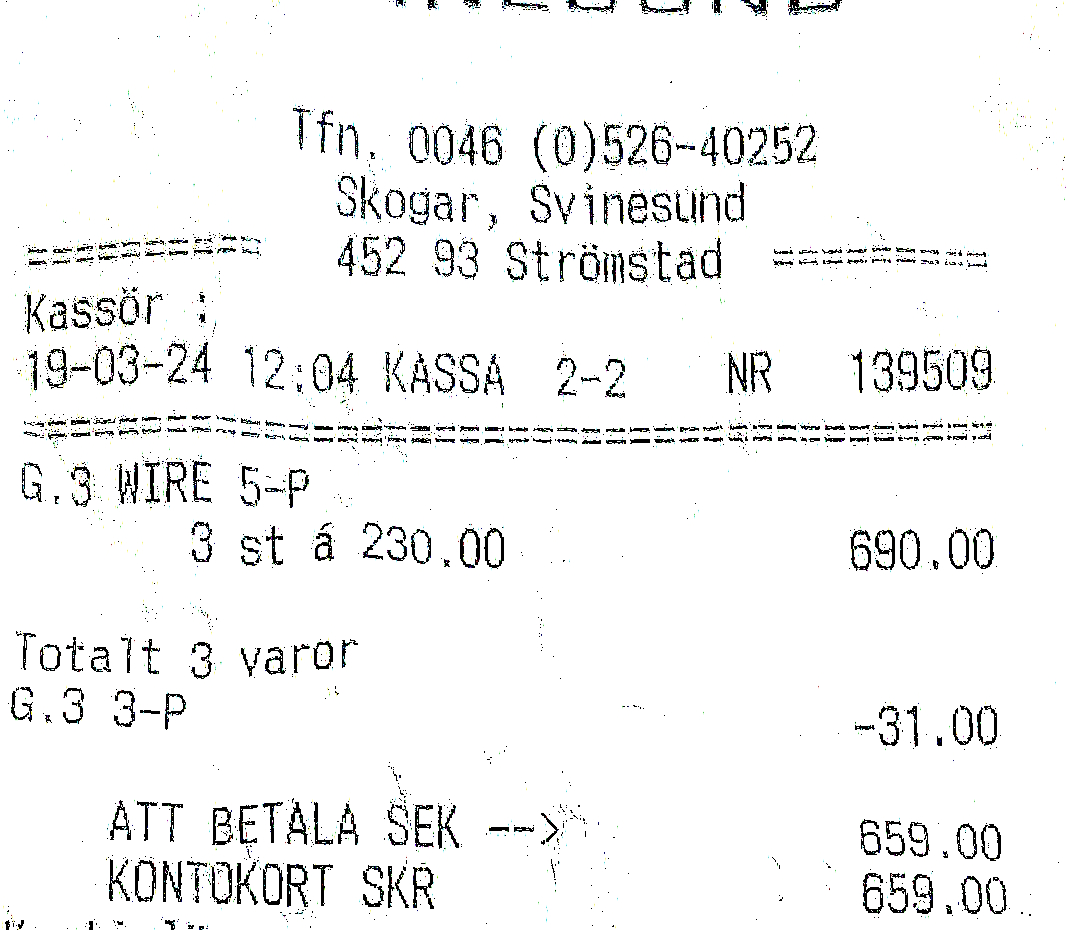
\includegraphics[scale=0.2]{images/test_image_threated.jpg}
\caption{Behandlet versjon av figur \ref{fig:kvittering}}
\label{fig:behandlet_kvittering}
\end{figure}
\footnote{https://docparser.com/blog/improve-ocr-accuracy/}


\section{Gjennomføring}
\subsection{Deskewing}
Et problem med å gjennomføre tekstgjenkjenning på et bilde uten å ha behandlet det først er at man ikke har noen garanti på at bilde har riktig vinkel. Hvis teksten ikke går parallelt med bilde vil resultatet kunne bli dårligere. Som observert i figur \ref{fig:skewed45} og figur \ref{fig:skewed10} har vi et bilde som er riktig orjentert og et bilde som er feil orientert. På bildet som er feil orientert klarer ikke tesseract å gjenkjenne teksten. På bildet som er rikitg orientert får vi følgende resultat som sett i figur \ref{fig:skewed10result}. Dette resultatet er bedre, men fortsatt langt fra treffsikkert.


\begin{figure}[h]
\centering
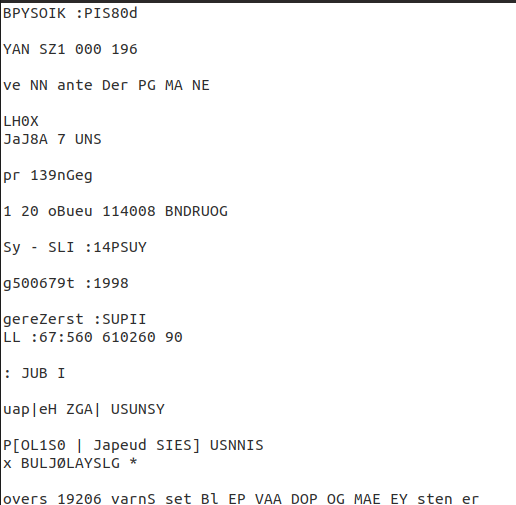
\includegraphics[scale=0.6]{images/skewed10results}
\caption{Resultate av tessearct OCR}
\label{fig:skewed10result}
\end{figure}


\begin{figure}[h]
\centering
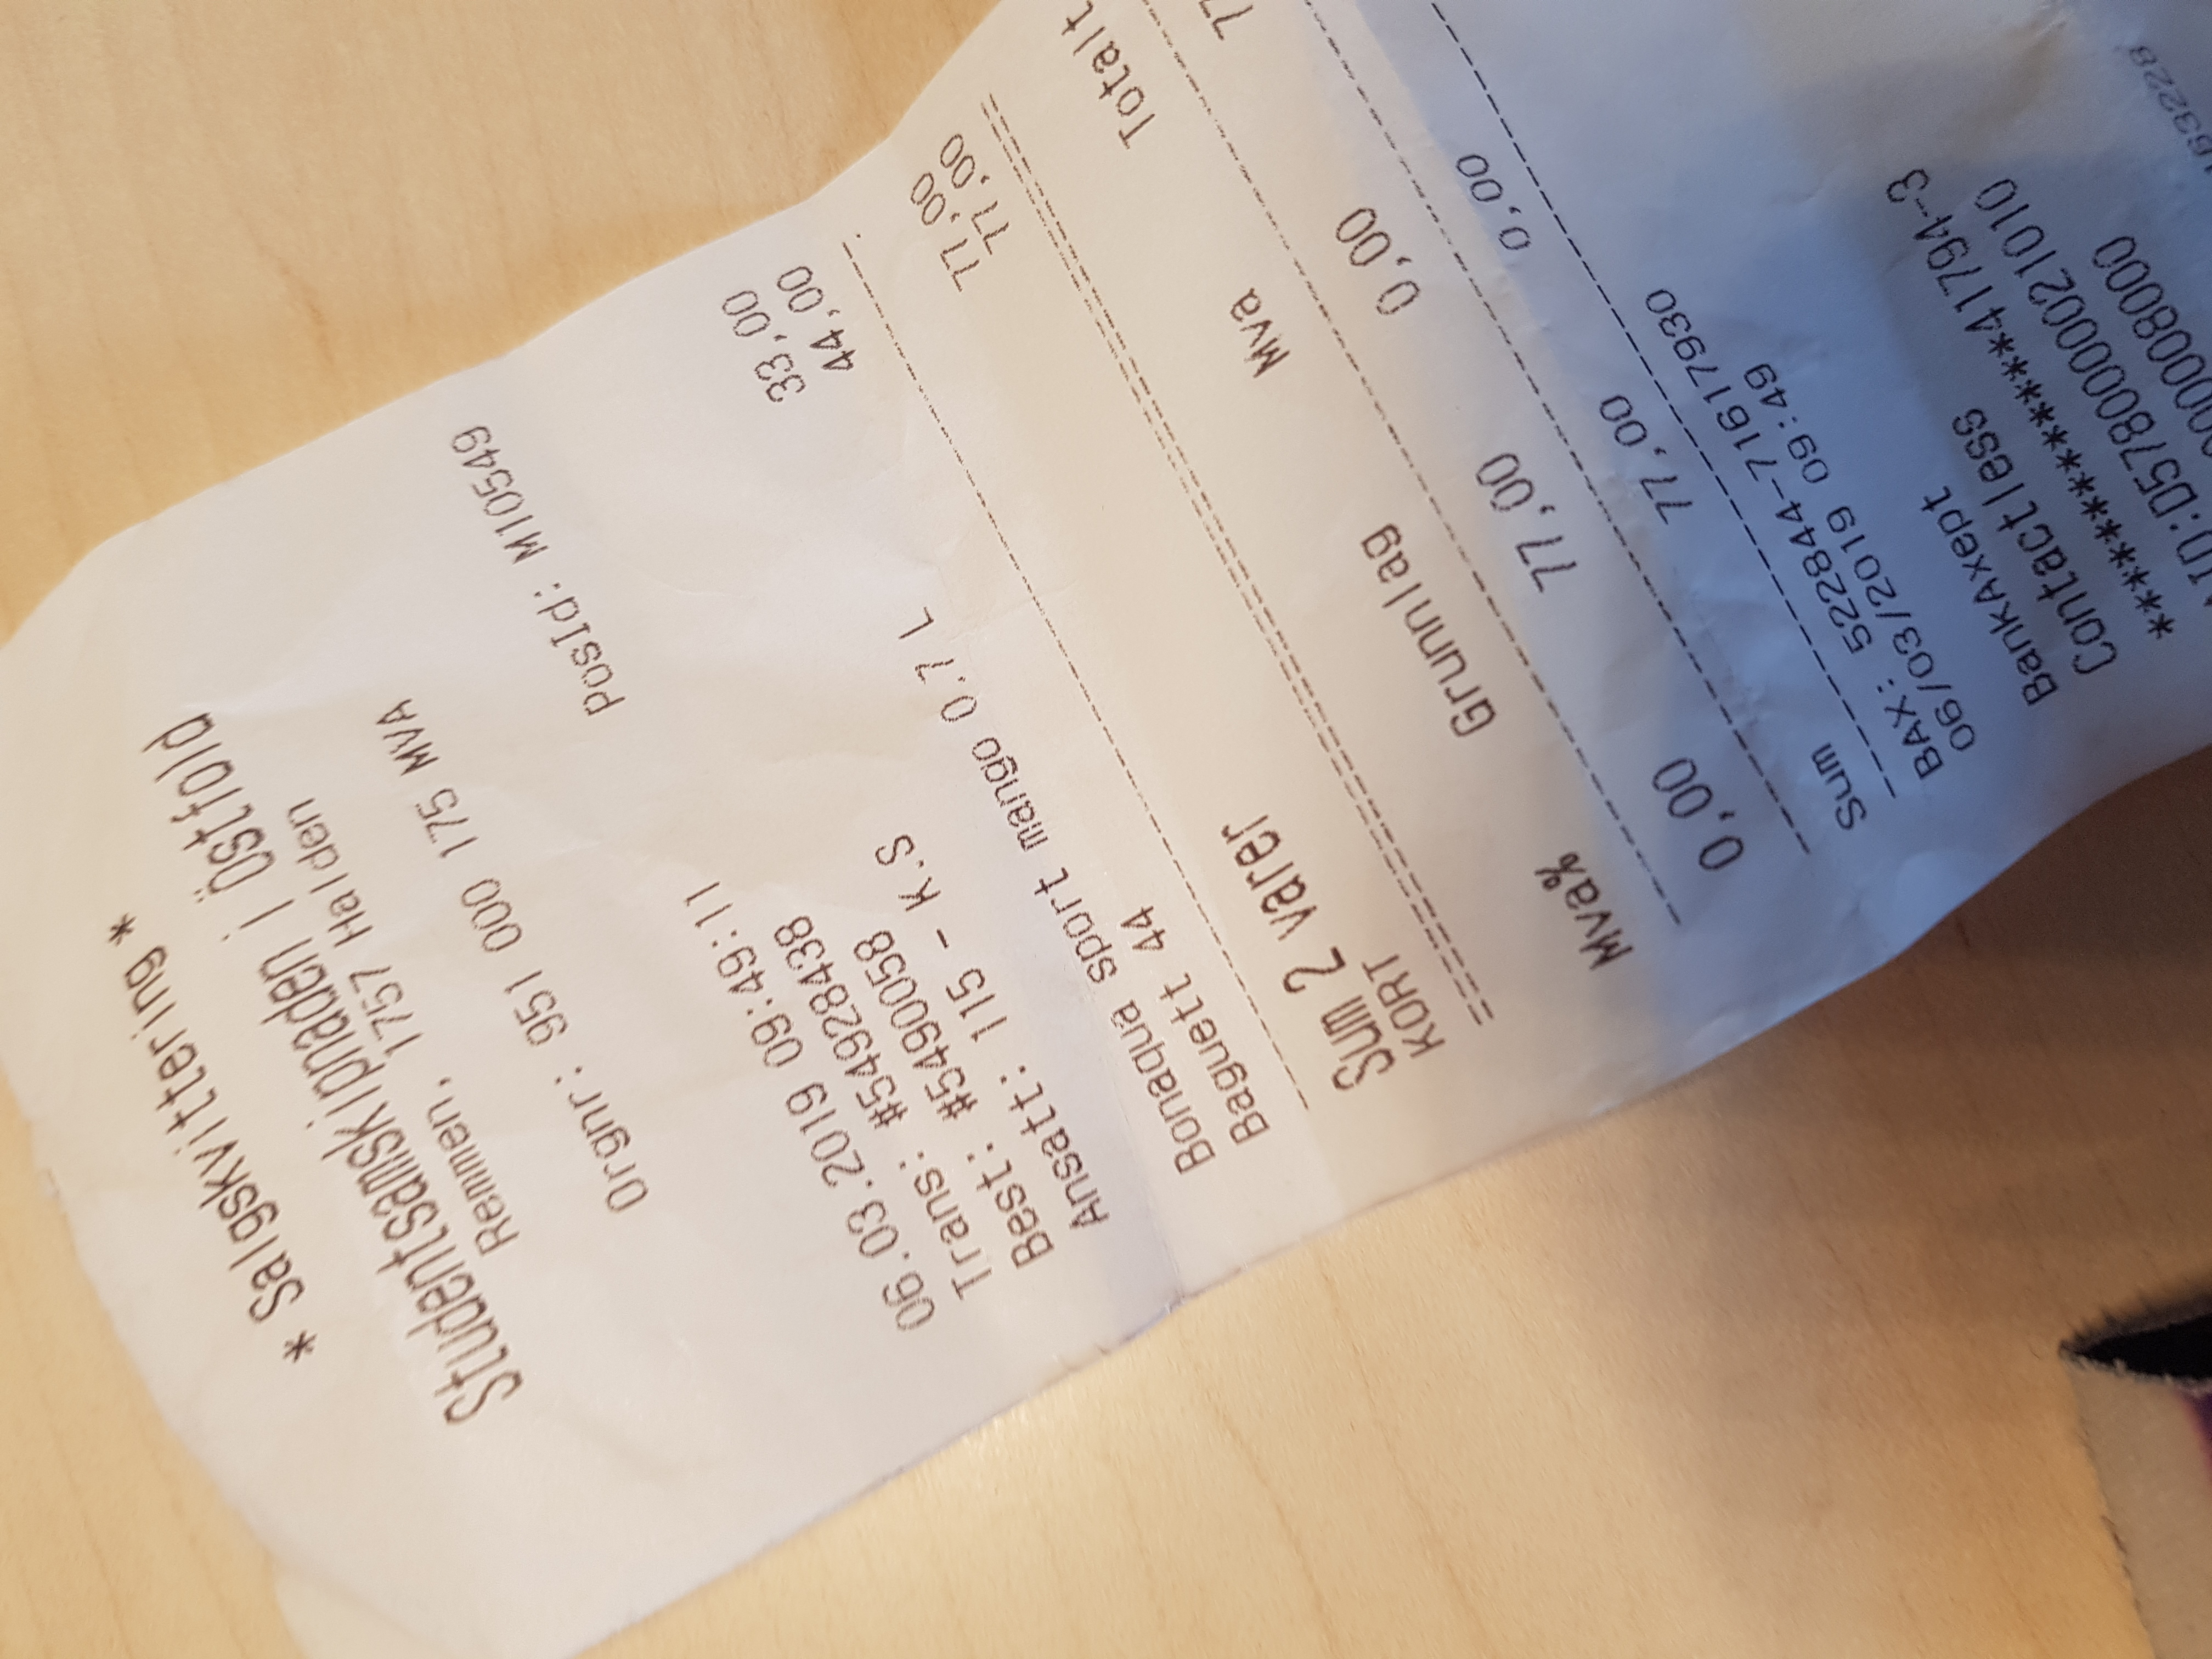
\includegraphics[scale=0.05, angle=270]{images/skewed45}
\caption{Bilde med feil rotering}
\label{fig:skewed45}
\end{figure}


\begin{figure}[h]
\centering
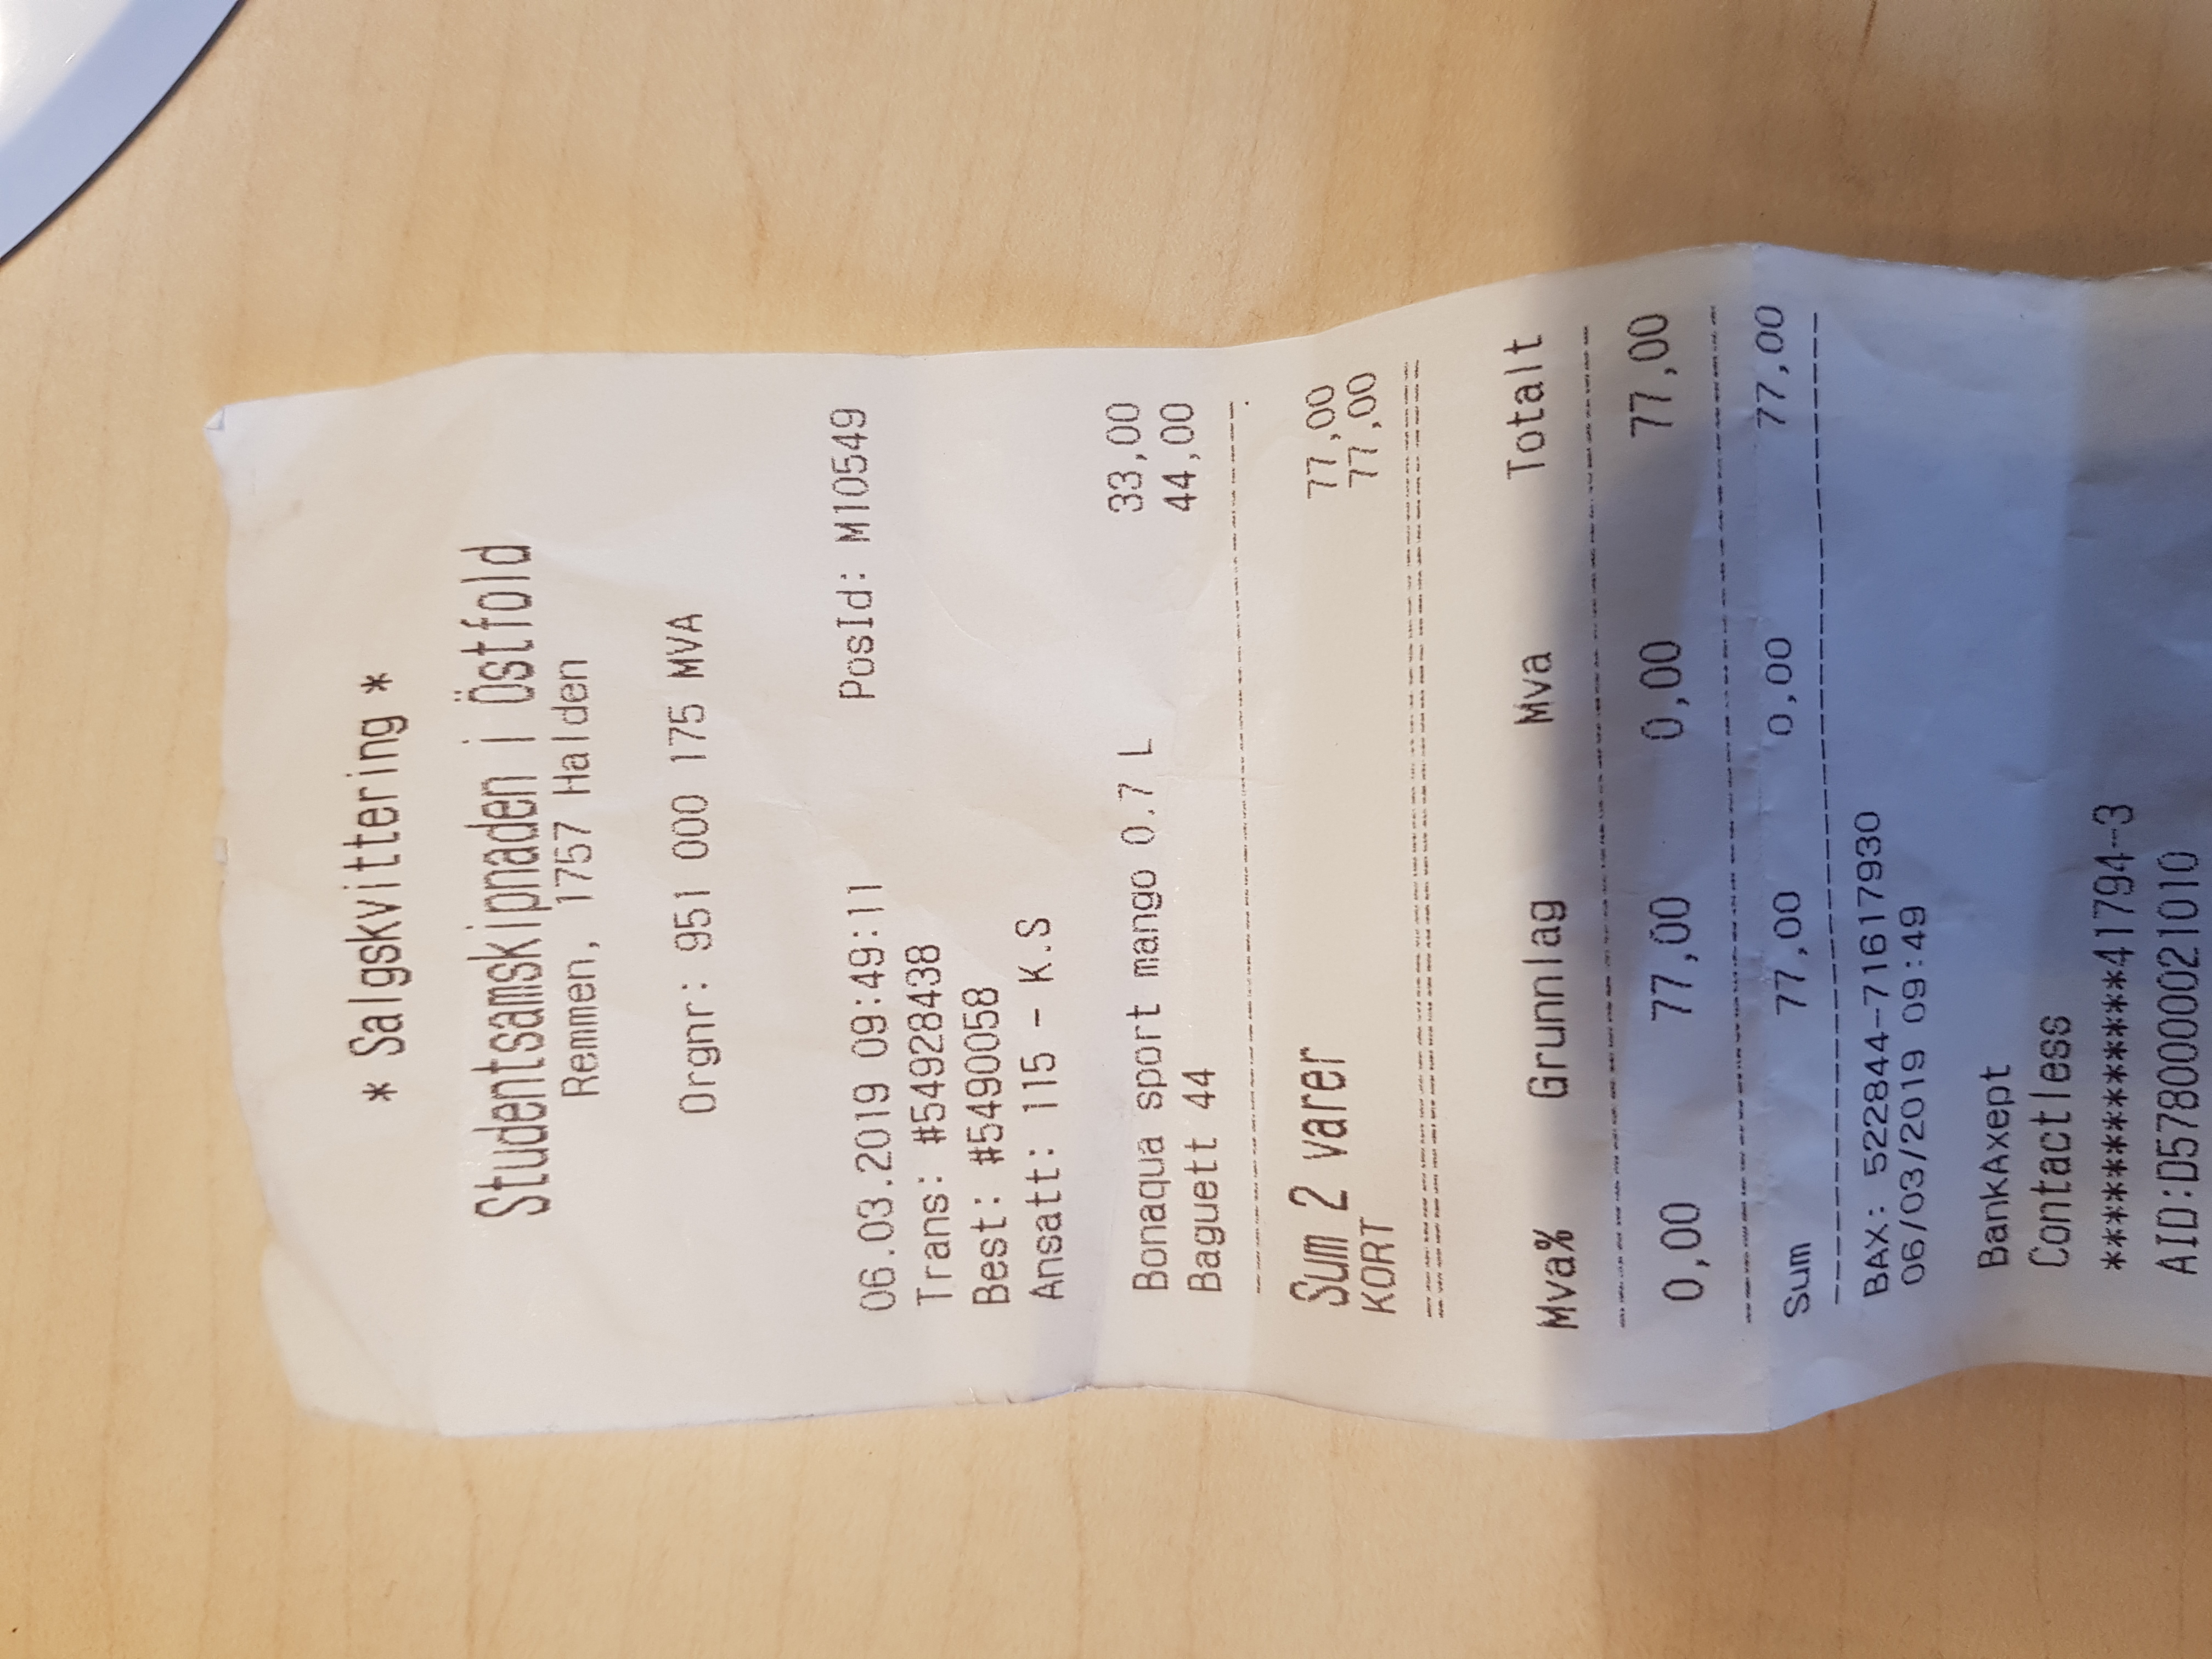
\includegraphics[scale=0.05, angle=270]{images/skewed10}
\caption{Bilde med riktig rotering}
\label{fig:skewed10}
\end{figure}

\paragraph{Hough}
Hough transformasjonen er brukt for å detektere former. Algoritmen har potensiale til å detektere forskjellige typer former, men i denne sammenhengen er den kun nyttig for å detektere linjer \footnote{https://en.wikipedia.org/wiki/Hough_transform#Implementation}. 
\paragraph{Linjeanalyse}
\paragraph{Homography}


\end{document}